\documentclass[conference]{IEEEtran}
\usepackage[spanish]{babel}
\usepackage[utf8]{inputenc}
\usepackage{blindtext, graphicx}
\usepackage{mdwmath}
\usepackage{mdwtab}

\begin{document}
\title{ Ajuste lineal y ecualizaci\'on del histograma de una imagen}
\author{\IEEEauthorblockN{Walter Alejandro Moreno Ram\'irez}
\IEEEauthorblockA{Departamento de Estudios Multidisciplinarios\\
Universidad de Guanajuato\\
Yuriria, Guanajuato\\
Correo: wa.morenoramirez@ugto.mx}}

\maketitle
\renewcommand\abstractname{Abstract}
\begin{abstract}
This article describes how to implement the linear adjustment and equalization of the histogram of an image with different contrast values. In addition to the relevance of such methods, as well as their advantages and disadvantages. \\\\
\end{abstract}

\begin{IEEEkeywords}
Pixel, histograma, histograma acumulado, curva tonal, brillo, contraste, funci\'on, C++, OpenCV.
\end{IEEEkeywords}

\IEEEpeerreviewmaketitle
\section{Introducci\'on}
Con el histograma obtenemos la distribuci\'on de grises en toda una imagen, si dicha distribuci\'on no es uniforme y se centra en un rango en espec\'ifico, se busca la mejor manera para corregir ese ``defecto'' que pueda tener la imagen, con el fin obtener mayor calidad de la misma.\\\\
Algo muy frecuente al momento de analizar fotograf\'ias es que pueden presentar un contraste incorrecto. Para probar los dos m\'etodos que se estudian y describen en \'este art\'iculo se utilizar\'an 3 im\'agenes, las cuales se ir\'an describiendo a continuaci\'on.\\
El histograma de una imagen muy oscura muestra una frecuencia de grises en un intervalo muy cercano al 0 como se puede ver en la Figura 1.

\begin{figure}[h]
	\begin{center}
		\setlength{\unitlength}{0.00105in}
		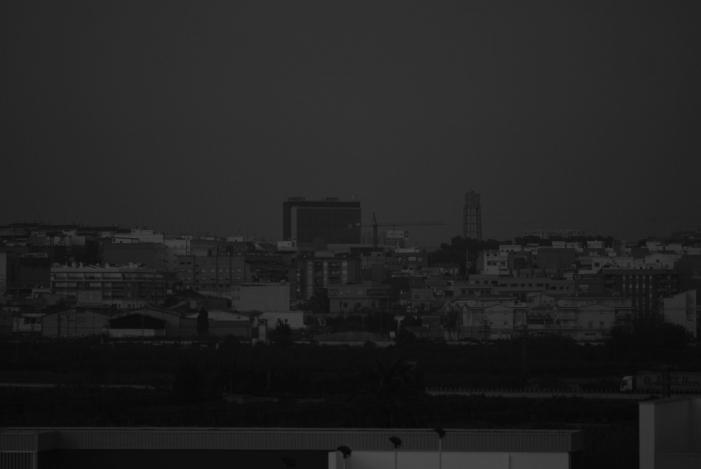
\includegraphics[scale=0.27]{./images/city.jpg}
		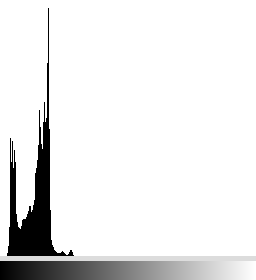
\includegraphics[scale=0.377]{./images/figure1_1.png}
	\end{center}
	\caption{\emph{ Imagen muy oscura y su respectivo histograma.}}
\end{figure}
En cambio, en una imagen con mucho brillo ese intervalo es m\'as cercano al 255 tal como se aprecia en la Figura 2.\\
\begin{figure}[h]
	\begin{center}
		\setlength{\unitlength}{0.00105in}
		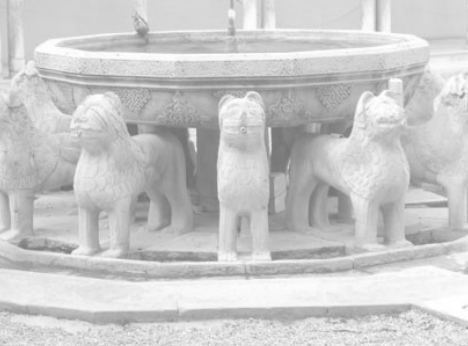
\includegraphics[scale=0.35]{./images/fuente.png}
		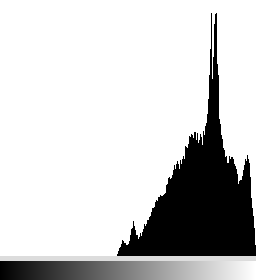
\includegraphics[scale=0.368]{./images/figure1_2.png}
	\end{center}
	\caption{\emph{ Imagen muy iluminada y su respectivo histograma.}}
\end{figure}
\newpage
En comparaci\'on con los histogramas de la Figura 1 y Figura 2, una imagen con alto contraste presenta dos intervalos, uno cerca del 0 y otro cercano al 255, con pocos medios tonos de grises. Lo anterior se puede apreciar mejor en la Figura 3.
\begin{figure}[h]
	\begin{center}
		\setlength{\unitlength}{0.00105in}
		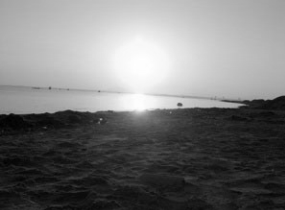
\includegraphics[scale=0.57]{./images/playa.png}
		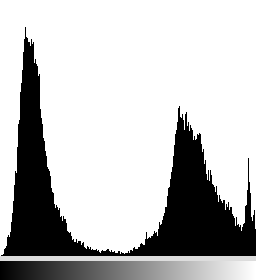
\includegraphics[scale=0.466]{./images/figure2_2.png}
	\end{center}
	\caption{\emph{ Imagen con un alto contraste y su histograma.}}
\end{figure}

Para corregir los ``defectos'' mencionados con anterioridad es necesario distribuir uniformemente en toda la imagen los intervalos que se aprecian en los histogramas, esto se puede lograr realizando operaciones sobre la imagen, como multiplicar por un valor definido todos los p\'ixels, esto da como resultado que el histograma se ``estire'' y se distribuyan mejor los colores, pero no es muy eficaz en todos los casos. Si queremos obtener buenos resultados es necesario realizar una transformaci\'on sobre la imagen.\\\\
Las transformaciones pueden verse como una funci\'on $f: N \rightarrow N$ donde f es cualquier funci\'on y se interpreta como: para cada valor de gris de entrada le corresponde un valor de salida.\\\\
Para corregir un contraste incorrecto se realizar\'an dos tipos de transformaciones al histograma: \textbf{\emph{ajuste lineal}} y \textbf{\emph{ecualizaci\'on}} .\\ La primer transformaci\'on, \textbf{\emph{ajuste lineal}} o \textbf{\emph{estiramiento (stretch)}} del histograma, se representa por la Ecuaci\'on (1).\\

\begin{equation}
	Im_{out}(i,j) = 255\left(\frac{Im_{in}(i,j)-Min}{Max-Min}\right)
\end{equation}
\\
Consiste en buscar el valor m\'inimo y el valor m\'aximo del histograma en la escala de grises de la imagen de antrada, realizando las operaciones indicadas en la Ecuaci\'on (1) sobre cada pixel en cada uno de los canales de la imagen.\\\\
Y la segunda transformaci\'on, \textbf{\emph{ecualizaci\'on}} del histograma, se logra obteniendo una curva tonal que represente como se puede ir distribuyendo cada intensidad de la escala de grises. Dicha curva se obtiene de un histograma acumulado y se representa por las Ecuaciones (2) y (3).\\
\begin{equation}
	H_{c}[0] = 0
\end{equation}

\begin{equation}
	H_{c}[P] = 	H_{c}[P-1]+	H_{c}[P]
\end{equation}

Esto es para $p=1,2,...,G-1$\\\\
Donde $H_c$ es el arreglo para el histograma acumulado, $P$ es el \'indice de cada elemento dentro del arreglo y G el n\'umero de elemntos del arreglo $H_c$.\\\\
Una vez tenemos el histograma acumulado  se utiliza la Ecuaci\'on (4) para obtener la funci\'on de transformaci\'on.\\
\begin{equation}
	T[P] = round\left( \frac{G-1}{MN}H_{c}[P]\right)
\end{equation}
Teniendo la funci\'on de transformaci\'on se reescribe la imagen de entrada para crear una imagen de salida con $g_p$ niveles de grises cambiando los valores de acuerdo a la Ecuacion (5).
\begin{equation}
	g_p = T[g_p]
\end{equation}
Ya que se explicaron ambos m\'etodos, se procede a continuar con la pr\'actica.\\

\section{Metodolog\'ia}
Tomando como referencia la pr\'actica anterior, se usar\'a el histograma que se genera para poder ajustar los tonos de grises de cada canal de la imagen.\\
Ambos programas fueron desarrollados en C++ usando las librerias de OpenCV para el procesamiento de im\'agenes.\\\\
En el programa base ya existian dos funciones; una para obtener el histograma de una imagen y la otra funci\'on se utiliza para crear una imagen y poder ``dibujar'' el histograma sobre ella.\\\\
Para realizar la pr\'actica se creo otra funci\'on y se nombr\'o \textbf{ajuste\_lineal}. Dicha funci\'on recibe como \'unico 
par\'ametro una imagen de tipo \textbf{Mat}, con la cual se trabajar\'a.\\

De la Ecuaci\'on (1) podemos reordenarla para que tome de la forma de la Ecuaci\'on (6).

\begin{equation}
	Im_{out}(i,j) = \left(\frac{255}{Max-Min}\right)\left(Im_{in}(i,j)-Min\right)
\end{equation}
\\
Cabe mencionar que tanto la Ecuaci\'on (1) como la Ecuaci\'on (6) matem\'aticamente son iguales, lo que se hizo fue cambiar la resta que se encuentra en el denominador y ponerlo como denominador de valor $255$, esto no afecta la ecuaci\'on ya que dicho valor multiplica a la fracci\'on completa.\\\\
De la Ecuaci\'on(6) podemos notar que el primer t\'ermino es una constante, por lo tanto, una vez obtenidos los valores Max y Min, se guarda en una variable con identificador \textbf{factor}. Lo anterior se realiza para facilitar las operaciones, ya que tambi\'en pueden ocasionar errores al momento de aplicar la ecuaci\'on.\\\\
Para poder aplicar el \textbf{ajuste\_lineal} primero se clona la imagen de prueba, para ello se utiliza la siguiente instrucci\'on:
\begin{center}
Mat newImage = image.clone();
\end{center}
donde el nuevo objeto \textbf{newImage} de tipo Mat tiene todas las caracter\'isticas del objeto \textbf{image}.\\
Una vez teniendo la imagen clonada, el valor de la variable \textbf{factor}, los valores Max, Min y de acuerdo al pseudoc\'odigo de la Figura 5. se procede a relizar el \textbf{ajuste\_lineal} al objeto \textbf{newImage}.

\begin{figure}[h]
	\begin{center}
		\setlength{\unitlength}{0.00105in}
		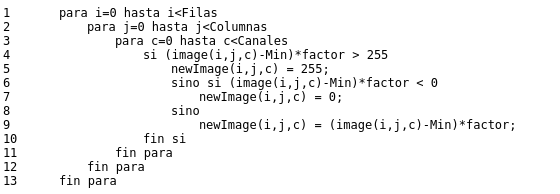
\includegraphics[scale=0.55]{./images/algoritmo.png}
	\end{center}
	\caption{Pseudoc\'odigo para realizar el \textbf{ajuste lineal} a una imagen.}
\end{figure}

%1		para i=0 hasta i<Filas
%2			para j=0 hasta j<Columnas
%3				para c=0 hasta c<Canales
%4					si (image(i,j,c)-Min)*factor > 255
%5						newImage(i,j,c) = 255;
%6						sino si (image(i,j,c)-Min)*factor < 0
%7							newImage(i,j,c) = 0;
%8 						sino
%9							newImage(i,j,c) = (image(i,j,c)-Min)*factor;
%10					fin si
%11				fin para
%12			fin para
%13		fin para

De acuerdo al pseudoc\'odigo de la Figura 5. cuando el valor resultante de la operaci\'on \textbf{(image(i,j,c)-Min)*factor} es mayor a 255 y menor a 0, los valores toman valores fuera de los rangos de la imagen, lo que se le conoce como overflow o desbordamiento. Al cumplirse tales condiciones, y la imagen al no poder contener valores negativos ni valores mayores de 255 los toma como valores positivos opuestos en la escala de grises. Lo anterior quiere decir que si existe un valor negativo se toma como un tono de gris muy claro o blanco, al igual si es un n\'umero mayor a 255 se toma como un gris muy oscuro o negro.\\ Un pixel por encima de los 255 o por debajo de 0 se dice que est\'a saturado y debido a esto se tienen que poner sus respectivos valores l\'imite mas cercanos sobre la imagen, como se realiza en la l\'inea 5 y 7 del pseudoc\'odigo. Si el valor calculado no es mayor a 255 o menor a 0 se ``dibuja'' en la imagen con su respectivo valor en cada canal.\\\\

\section{Resultados}
Como primer prueba se utiliza una foto muy poco luminosa. Con valores $Min=10$ y $Max=50$ de acuerdo a su histograma, el resultado de la imagen de la Figura 1. aplicandole el ajuste lineal se muestra en la Figura 6.\\\\
\begin{figure}[h]
	\begin{center}
		\setlength{\unitlength}{0.00105in}
		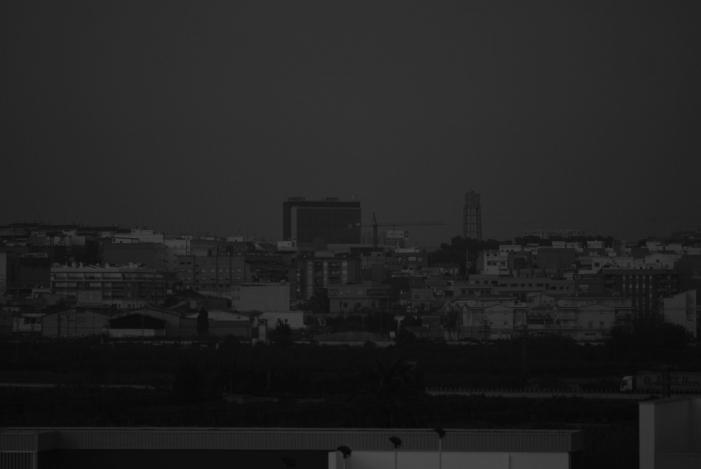
\includegraphics[scale=0.23]{./images/city.jpg}
		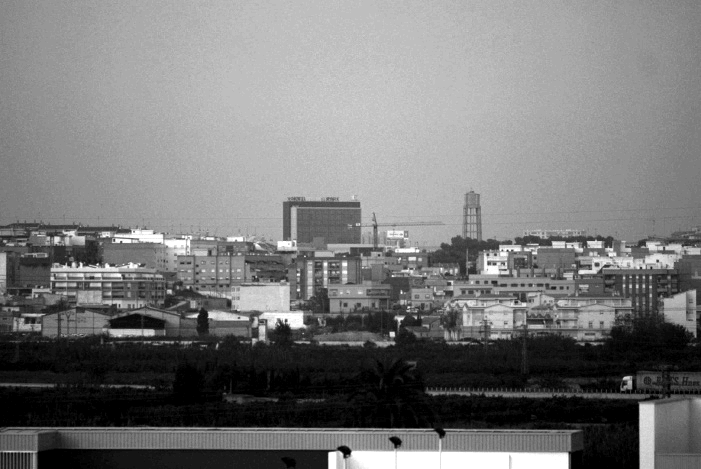
\includegraphics[scale=0.2298]{./images/city_out.png}
	\end{center}
	\caption{Imagen original e imagen aplicandole el ajuste lineal, respectivamente.}
\end{figure}

Como segunda prueba se utiliza una foto muy luminosa. Con valores $Min=140$ y $Max=255$ de acuerdo a su histograma, el resultado de la imagen de la Figura 2. aplicandole el ajuste lineal se muestra en la Figura 7.

\begin{figure}[h]
	\begin{center}
		\setlength{\unitlength}{0.00105in}
		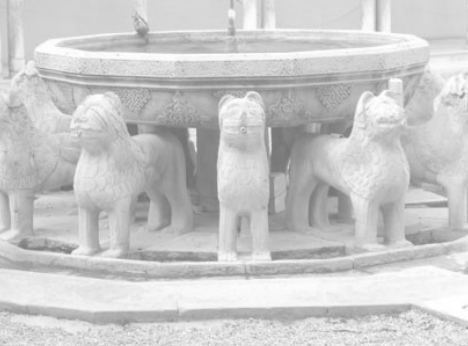
\includegraphics[scale=0.335]{./images/fuente.png}
		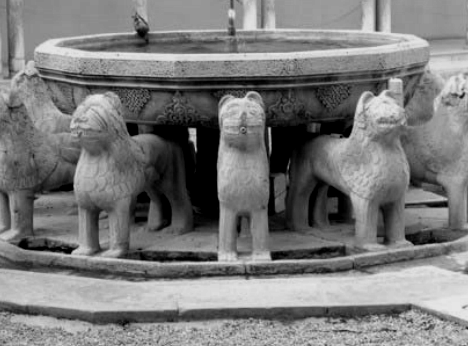
\includegraphics[scale=0.334]{./images/fuente_out.png}
	\end{center}
	\caption{Imagen original e imagen aplicandole el ajuste lineal, respectivamente.}
\end{figure}

Para la imagen de la Figura 3, aplicando el ajuste lineal con valores $Min=20$ y $Max=230$ su resultado se muestra en la figura 8.
\begin{figure}[h]
	\begin{center}
		\setlength{\unitlength}{0.00105in}
		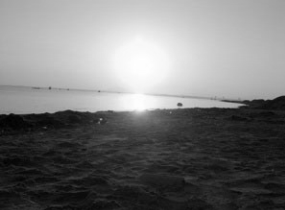
\includegraphics[scale=0.50]{./images/playa.png}
		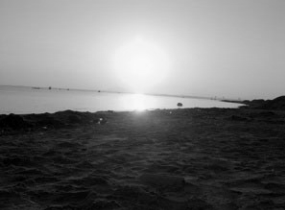
\includegraphics[scale=0.50]{./images/playa_out.png}
	\end{center}
	\caption{Imagen original e imagen aplicandole el ajuste lineal, respectivamente.}
\end{figure}

Para realizar la ecualizaci\'on del histograma primeramente se obtiene el histograma acumulado. Ya que en la Ecuacion (2) el primer elemento del arreglo es cero, cuando el contador $i$ tome el valor $0$ se hace la acci\'on indicada en dicha ecuaci\'on. Para el primer elemento descrito anteriormente y los consecuentes elementos se descrien mediante el pseudoc\'odigo que se muestra en la Figura 8.

\begin{figure}[h]
	\begin{center}
		\setlength{\unitlength}{0.00105in}
		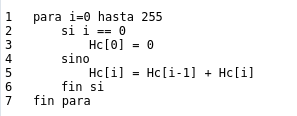
\includegraphics[scale=0.50]{./images/algoritmo2.png}
	\end{center}
	\caption{Pseudoc\'odigo para obtener el histograma acumulado.}
\end{figure}

%1	para i=0 hasta 255
%2		si i == 0
%3 			Hc[0] = 0
%4		sino
%5			Hc[i] = Hc[i-1] + Hc[i]
%6		fin si
%7 	fin para
Una vez se tiene el histograma acumulado y de acuerdo a la Ecuaci\'on (4) se obtiene la funci\'on de transformaci\'on para la imagen.\\
A continuaci\'on se mostrar\'an los resultados obtenidos con las imagenes de prueba, tanto el histograma acumulado que nos da la curva tonal, como su funci\'on de transformaci\'on.\\

Primer imagen de prueba.
\begin{figure}[h]
	\begin{center}
		\setlength{\unitlength}{0.00105in}
		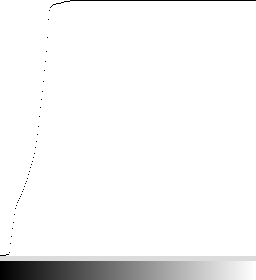
\includegraphics[scale=0.50]{./images/Ha1.png}
		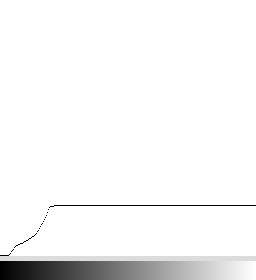
\includegraphics[scale=0.50]{./images/Ha1_1.png}
	\end{center}
	\caption{Curva tonal y funci\'on de transformaci\'on respectivamente, para la primer imagen.}
\end{figure}

Segunda imagen de prueba.
\begin{figure}[h]
	\begin{center}
		\setlength{\unitlength}{0.00105in}
		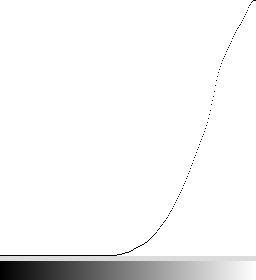
\includegraphics[scale=0.50]{./images/Ha2_1.png}
		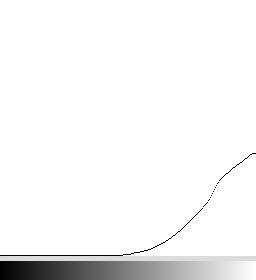
\includegraphics[scale=0.50]{./images/Ha2_2.png}
	\end{center}
	\caption{Curva tonal y funci\'on de transformaci\'on respectivamente, para la primer imagen.}
\end{figure}
\newpage
Y por \'ultimo la tercer imagen de prueba.
\begin{figure}[h]
	\begin{center}
		\setlength{\unitlength}{0.00105in}
		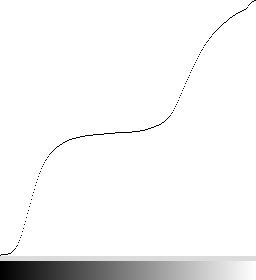
\includegraphics[scale=0.50]{./images/Ha3_1.png}
		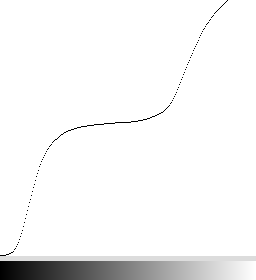
\includegraphics[scale=0.50]{./images/Ha3_2.png}
	\end{center}
	\caption{Curva tonal y funci\'on de transformaci\'on respectivamente, para la primer imagen.}
\end{figure}

Un detalle que es debido aclarar es que el histograma acumualdo, para una mejor proyecci\'on en las gr\'aficas, se normalizo igual que el histograma. Primero se dividieron todos los elementos entre el valor mayor, que se encuentra la posici\'on 255 del histograma, posteriormente se realiz\'o el producto entre cada elemento del arreglo del histograma acumulado por 255, para dar un l\'imite de altura, ya que la imagen que se cre\'o para mostrar los histogramas, como m\'axima altura tienes 255 p\'ixeles.\\\\

\section{Concluciones}
Aunque es una t\'ecnica que da buenos resultados tiene una desventaja muy importante, ya que si la concentraci\'on de tonos de grises se encuentra en ambos extremos del histograma y escogemos como m\'inimo y m\'aximo los l\'imites de la escala de grises, 0 y 255, al aplicar la transformaci\'on la imagen no sufre cambio alguno. La explicaci\'on  es porque al realizar la divisi\'on $\frac{255}{Max-Min}$, siendo $Max=255$ y $Min=0$, el resultado es $1$. Con este resultado nos damos cuenta que no se realiza ning\'un cambio, siendo la imagen de salida igual a la imagen de entrada.\\\\
En lo que respecta a la ecualizaci\'on del histograma, cuando se obtiene la funci\'on de transformaci\'on es m\'as seguro que se producir\'a un cambio o correci\'on de ciertos ``defectos'', aunque tambi\'en tiene sus defectos ya que en algunos casos los resultados pueden ser artificiosos.
%\begin{thebibliography}{1}
%    \bibitem{IEEEhowto:kopka}
%    H.~Kopka and P.~W. Daly, \emph{A Guide to \LaTeX}, 3rd~ed.\hskip 1em plus
%      0.5em minus 0.4em\relax Harlow, England: Addison-Wesley, 1999.
%\end{thebibliography}

%\begin{IEEEbiography}[{\includegraphics[width=1in,height=1.25in,clip,keepaspe%ctratio]{picture}}]{John Doe}
%\blindtext
%\end{IEEEbiography}

\end{document}